%----------------------------------------------------------------
%
%  File    :  thesis.tex
%
%  Authors :  Keith Andrews, IICM, TU Graz, Austria
%             Manuel Koschuch, FH Campus Wien, Austria
%			  Sebastian Ukleja, FH Campus Wien, Austria
% 
%  Created :  22 Feb 96
% 
%  Changed :  14 Oct 2020
%
%  For suggestions and remarks write to: sebastian.ukleja@fh-campuswien.ac.at
% 
%----------------------------------------------------------------

% --- Setup for the document ------------------------------------

%Class for a book like style:
\documentclass[11pt,a4paper,oneside]{scrbook}
%For a more paper like style use this class instead:
%\documentclass[11pt,a4paper,oneside]{thesis}

%input encoding for windows in utf-8 needed for Ä,Ö,Ü etc..:
\usepackage[utf8]{inputenc}
%input encoding for linux:
%\usepackage[latin1]{inputenc}
%input encoding for mac:
%\usepackage[applemac]{inputenc}

\usepackage[english]{babel}
% for german use this line instead:
%\usepackage[ngerman]{babel}

%needed for font encoding
\usepackage[T1]{fontenc}

%Package for floating figures
\usepackage{float}

% want Arial? uncomment next two lines...
%\usepackage{uarial}
%\renewcommand{\familydefault}{\sfdefault}

% BIBLOGRAPHY
\usepackage{biblatex}
\addbibresource{testBib.bib}

%some formatting packages
\usepackage[bf,sf]{subfigure}
\renewcommand{\subfigtopskip}{0mm}
\renewcommand{\subfigcapmargin}{0mm}

%For better font resolution in pdf files
\usepackage{lmodern}

\usepackage{url}

%\usepackage{latexsym}

\usepackage{geometry} % define pagesize in more detail


\usepackage{colortbl} % define colored backgrounds for tables

\usepackage{biblatex}

\usepackage{courier} %for listings
\usepackage{listings} % nicer code formatting
\lstset{basicstyle=\ttfamily,breaklines=true}

\usepackage{graphicx}
  \pdfcompresslevel=9
  \pdfpageheight=297mm
  \pdfpagewidth=210mm
  \usepackage[         % hyperref should be last package loaded
    pdftex, 		   % needed for pdf compiling, DO NOT compile with LaTeX
    bookmarks,
    bookmarksnumbered,
    linktocpage,
    pdfview={Fit},
    pdfstartview={Fit},
    pdfpagemode=UseOutlines,                 % open bookmarks in Acrobat
  ]{hyperref}
\DeclareGraphicsExtensions{.pdf,.jpg,.png}
\usepackage{bookmark}

\usepackage[title]{appendix}

%paper format
\geometry{a4paper,left=30mm,right=25mm, top=30mm, bottom=30mm}

% --- Settings for header and footer ---------------------------------
\usepackage{scrlayer-scrpage}
\clearscrheadfoot
\pagestyle{scrheadings}
\automark{chapter}

%Left header shows chapter and chapter name, will not display on first chapter page use \ihead*{\leftmark} to show on every page
\ihead{\leftmark} 	
%\ohead*{\rightmark}	%optional right header
\ifoot*{Gabriel Karl Hübner}		%left footer shows student name
\ofoot*{\thepage}		%right footer shows pagination
%---------------------------------------------------------------------

%Start of your document beginning with title page
\begin{document}


% --- Main Title Page ------------------------------------------------
\begin{titlepage}
\frontmatter

\begin{picture}(50,50)
\put(-70,40){\hbox{
\includegraphics{images/logo.png}}}
\end{picture}

\vspace*{-5.8cm}

\begin{center}

\vspace{6.2cm}

\hspace*{-1.0cm} {\LARGE \textbf{Web 3.0\\}}
\vspace{0.2cm}
\hspace*{-1.0cm} Challenges and Opportunities from the perspective of blockchain technologies\\

\vspace{2.0cm}

\hspace*{-1.0cm} { \textbf{Bachelor Thesis\\}}

\vspace{0.65cm}

\hspace*{-1.0cm} Submitted in partial fulfillment of the requirements for the degree of \\

\vspace{0.65cm}

\hspace*{-1.0cm} \textbf{Bachelor of Science in Engineering\\}

\vspace{0.65cm}

\hspace*{-1.0cm} to the University of Applied Sciences FH Campus Wien \\
\vspace{0.2cm}
\hspace*{-1.0cm} Bachelor Degree Program: Computer Science and Digital Communications \\

\vspace{1.6cm}

\hspace*{-1.0cm} \textbf{Author:} \\
\vspace{0.2cm}
\hspace*{-1.0cm} Gabriel Karl Hübner \\

\vspace{0.7cm}

\hspace*{-1.0cm} \textbf{Student identification number:}\\
\vspace{0.2cm}
\hspace*{-1.0cm} 2010475105, 01408046\\

\vspace{0.7cm}

\hspace*{-1.0cm} \textbf{Supervisor:} \\
\vspace{0.2cm}
\hspace*{-1.0cm} BSc MSc Leon Freudenthaler \\

\vspace{0.7cm}

% Reviewer if needed
%\hspace*{-1.0cm} \textbf{Reviewer: (optional)} \\
%\vspace{0.2cm}
%\hspace*{-1.0cm} Title first name surname \\


\vspace{1.0cm}

\hspace*{-1.0cm} \textbf{Date:} \\
\vspace{0.2cm}
\hspace*{-1.0cm} dd.mm.yyyy \\

\end{center}
\end{titlepage}

\newpage

\vspace*{16cm}
\setcounter{page}{1}

% --- Declaration of authorship ------------------------------------------
\hspace*{-0.7cm} \underline{Declaration of authorship:}\\\\
I declare that this Bachelor Thesis has been written by myself. I have not used any other than the listed sources, nor have I received any unauthorized help.\\\\
I hereby certify that I have not submitted this Bachelor Thesis in any form (to a reviewer for assessment) either in Austria or abroad.\\\\
Furthermore, I assure that the (printed and electronic) copies I have submitted are identical.
\\\\\\
Date: \hspace{6cm} Signature:\\

% --- English Abstract ----------------------------------------------------
\cleardoublepage
\chapter*{Abstract}
Through the popularity of cryptocurrency, blockchain technologies have gained a lot of traction. These technologies play a huge part in the Web 3.0, as they are able to make decentralised applications possible. The current web is based on mostly centralised networks, which puts a lot of data into the hands of major corporations, such as Google. The decentralised web, could help users to gain full ownership of their own private data. This Bachelor thesis will explain what the Web 3.0 could be and what role blockchain technologies play in order to achieve this goal.\\\\


% --- German Abstract ----------------------------------------------------
\cleardoublepage
\chapter*{Kurzfassung}
(Z.B. ``Diese Arbeit untersucht...'')


% --- Abbrevations ----------------------------------------------------
\chapter*{List of Abbreviations}
\vspace{0.65cm}

DApp    - Decentralised Application\\
PoS     - Proof of Stake\\
PoW     - Proof of Work

% --- Key terms ----------------------------------------------------
\newpage
\chapter*{Key Terms}
\vspace{0.65cm}

\begin{itemize}
	\setlength{\itemsep}{0pt}
        \item[] Blockchain
        \item[] DApps
        \item[] Decentralization
        \item[] Smart contracts
        \item[] Web 3.0
\end{itemize}

% --- Table of contents autogenerated ------------------------------------
\newpage
\setcounter{tocdepth}{3}
\tableofcontents
\thispagestyle{empty}

% --- Begin of Thesis ----------------------------------------------------
\mainmatter
\chapter{Introduction}
\label{chap:intro}

In recent years, especially through the development of cryptocurrencies and blockchain technology, the term "Web 3.0" (sometimes also referred to as the semantic web and the next generation of the web) has gained more and more traction. The Web 3.0 is the next generation of the web after the web 2.0. The definition of this web is not clear at the time\cite{techtarget}. However there are several goals the Web 3.0 is meant to achieve, such as openness and  decentralization\cite{avast}. This Bachelor thesis will present some of the definitions for the Web 3.0 and the history of the web from web 1.0 to Web 3.0. The main focus of this Bachelor thesis is on one of the technologies that is part of the next generation of the web, the blockchain. The Bachelor thesis will explain the blockchain technology and some of the related technologies, such as "smart contracts" and "DApps". Then it will list some of the challenges, that the Web 3.0 and blockchains still have to face, as well as possible applications of the blockchain technology. The questions this Bachelor thesis wants to answer, are therefore: What is the Web 3.0? What are its challenges and opportunities, from the perspective of blockchain technologies?

\subsection{Contribution}

This Bachelor thesis contributes to a better understanding of the Web 3.0, as well as blockchain technologies. It will show, which problems still exist, that need to be overcome, before these technologies can be properly implemented. There are also many possible applications for blockchains in different fields. This Bachelor thesis will present some of the most popular applications, that can be implemented with blockchain technologies.

\subsection{Relevance}

Many users are not happy with the way their data is handled in the current web 2.0. Big corporations such as Google collect massive amounts of user data, to display personal tailored advertisements, in order to achieve higher profits\cite{nbcgoogle}. The decentralization of the web can improve upon that aspect and help users to protect their personal data. Blockchains are generally run in peer-to-peer networks, that are usually fully transparent, immutable and offer better privacy to users than centralised networks\cite{ibmblockchainadvantages}\cite{blockchaingeneral}. Users can benefit from these aspects, because they can see exactly who has accessed their data. With certain protocols in place, users can potentially even manage, who can access their personal data.\\
There are also many other fields, where blockchain technologies could improve upon current data management systems. It is therefore relevant to educate on some of the aspects of the next generation of the web, not just for users who want better privacy, but also for developers, who want to improve the web, by writing better applications for it.

\subsection{State of the Art}
The current state of the art is the web 2.0. This has the property of being a "read-write" web, where most of the content is generated by users. This is in contrast to the web 1.0, where most pages were "read-only". The web is described as a web of "rich user experiences" by Tim O'Reilly\cite{oreilly2007}. One of the main enablers for our current web is the technology AJAX. This made it possible to develop websites, that users can interact with, such as the social-media network Facebook. The current web is dominated by big corporations, such as Google and user data is generally saved on centralised servers. However some decentralised applications already exist, such as the ethereum network\cite{ethereumvision}, which is used to mine and trade cryptocurrencies.

\subsection{Methodology}

The methodology used in this Bachelor thesis, is that of a literature review. Multiple sources have been searched and examined, not only scientific, peer-reviewed papers, but also online sources, to get a better grasp on the topic. Google, Google Scholar and the IEEE Explorer were used to find sources for this Bachelor thesis. The search terms used to find sources were "Web 3.0", "Blockchain technology", "Web 3.0 challenges and opportunities", "Blockchain applications" and many other similar queries. The resulting sources were then carefully examined and used in different sections of the Bachelor thesis.

\subsection{Outlook}
This Bachelor thesis starts by giving a brief history of the web. After that, the many different definitions for the Web 3.0 are presented. Then the blockchain technology, as well as several related technologies, will be explained. The Bachelor thesis then continues to give some examples of the challenges blockchain technologies and the Web 3.0 have to face. In the last part, some of the possible applications of blockchain technologies are given.

\newpage
\chapter{Related Work}
This Bachelor thesis is composed of many different papers, which also deal with the opportunities and challenges of Web 3.0/blockchain technologies. This section lists the most relevant sources, that were used to write this Bachelor thesis.\\

The paper "An Overview of Blockchain Technology: Architecture, Consensus,
and Future Trends" \cite{blockchaingeneral} offers a good overview of how blockchains work. It has a focus on blockchains for cryptocurrency applications, but many concepts remain the same for other types of applications. This paper is used in chapter 3.1 "Blockchain technology".

There are several papers, that are used in chapter 4 "Challenges of the Web 3.0" and chapter 5 "Opportunities of the Web 3.0". However, the most noteworthy paper would be "A Survey of Blockchain From the Perspectives of Applications, Challenges, and Opportunities" \cite{challengesandapplications2019}. This paper offers a great outline for the challenges and opportunities of blockchain technologies. The paper describes challenges of blockchain technologies regarding performance and scalability, privacy, interoperability, energy consumption, fairness and security and current regulation problems. It also mentions possible fields of applications for blockchain technologies, such as healthcare, the energy industry, the stock market, voting, insurance, identity management and trade finance. Some of these challenges and applications will be expanded with more recent findings and different perspectives in this Bachelor thesis.

\newpage
\chapter{Web 3.0}
The first question, that emerges, when talking about the Web 3.0 (also called the Web3), is what it is by definition. There is neither an easy, nor a precise answer to that question, since there are many different definitions of the term. To better understand what the Web 3.0 is and what the term stands for, we can analyse the history of the two previous iterations of the web, the web 1.0 and web 2.0.

\section{History of the Web}
First of, it is important to understand, that the evolution of the web 1.0 to the web 2.0 did not take place at a concrete time. It was rather a slow progress, where certain websites gradually implemented additional functionalities and technologies, eg. AJAX. \cite{oreilly2007}\\

\textbf{Web 1.0}\\

The first "packet-switched" network, the ARPANET (Advanced Research Project Agency Network), was created in 1969 in the United States. This network connected four Universities and was one of the earliest forms of the internet. To accommodate for an open-architecture network environment Robert Kahn formalised the Transmission Control Protocol/Internet Protocol (TCP/IP), which was then implemented by Ray Tomlinso and Peter Kirstein. In the 1980´s Bob Metcalfe developed Ethernet Technology to connect a number of hosts in Local Area Networks (LANs). Later the Domain Name System (DNS) was invented by Paul Mockapetris to resolve host names into IP addresses. With these protocols, the basic building blocks of the internet were laid out.\cite{arxiv.org}\\

The "world-wide web" or web for short, has been established by Tim Burners-Lee in late 1989. This were static websites, which allowed users to read information and jump to different sites with the use of hyperlinks. In this sense, the web 1.0 was mostly a "read-only" web. This iteration of the web lasted until roughly 2005, when the web 2.0 was introduced.\cite{hiremath2016}\\
Figure 2.1 depicts a screenshot of the "first website", which was recreated and is hosted on \href{http://info.cern.ch/hypertext/WWW/TheProject.html}{info.cern.ch}.

\begin{figure}[H]
	\centering
		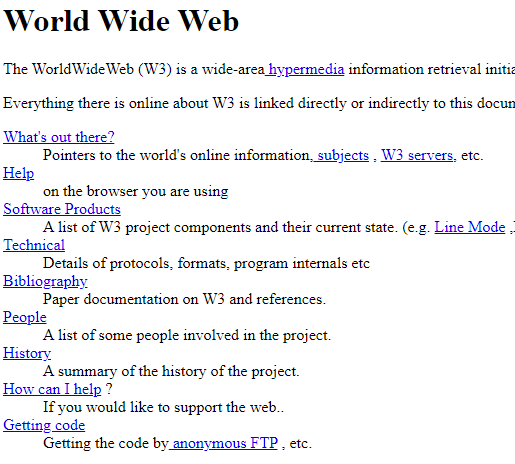
\includegraphics[width=12cm,keepaspectratio]{images/first_website.png}
	\caption{First Website from \href{http://info.cern.ch/hypertext/WWW/TheProject.html}{info.cern.ch}}
	\label{fig:first-website}
\end{figure}

\textbf{Web 2.0}\\\\
The term for the web 2.0 was first coined in 2004 by Dale Dougherty and Craig Cline in a conference with Tim O'Reilly. The key difference to the first iteration of the web, is that the second web allows read and write access instead of mostly read access. This could also be described as the first "dynamic" web, in contrast to the "static" web 1.0. Through "social-media" websites, "blogs", etc. users can generate content on a website, this leads to the terms "participative" web and "people-centric" web, for the web 2.0. \cite{hiremath2016}
Tim O'Reilly describes the web 2.0 as network with "rich user experiences", which are provided by websites from major corporations, such as the Google search engine. One of the key components is AJAX, which is composed of several technologies, such as XHTML and CSS to represent the data on website, the Document Object Model, XML and XSLT, XMLHttpRequest for asynchronous data retrieval and JavaScript to bind everything together.\cite{oreilly2007}
Nowadays there are of course several other or newer technologies and further developments of the web 2.0, however the core-concepts remain roughly the same.
This chapter should provide a general understanding of the history of the web, as well as a demarcation of the web 2.0 to the Web 3.0.
The next chapter will introduce a definition, as well as new technologies of the Web 3.0. \\

\section{Definition of Web 3.0}
Defining Web 3.0 is a challenging task. The availability of scientific papers in regard of the definition of Web 3.0 is relatively sparse, therefore online sources have been used.\\
As of now there is no concise definition for the third generation of the web to be found, since it is still being defined and evolving\cite{techtarget}.
When searching for the definition of the Web 3.0, it is often also called the semantic web, the transcendent web and the web of things\cite{definingweb3}. In this Bachelor thesis it will be described as the Web 3.0 or the new/next generation of the web. In contrast to the web 2.0, where data is created by humans, it is described as a web, where data is created by computers/machines. \cite{definingweb3}
As a side note, the term "semantic web" often seems confusing, because it is sometimes used as a synonym for the Web 3.0. This term was coined by Tim Berners-Lee, who predicted the possibility of computers to exchange semantic data.\cite{newmedia}
In this Bachelor thesis, the "semantic web" is not equal to the Web 3.0, it is rather a technology that is incorporated into it.\cite{avast}\\
The metadata (semantic data) in the semantic web, is data which describes data, so that it can be used/categorised by a computer. It can be used to optimize search engines, as well as a variety of other fields. \cite{CLARKE201279}\\
However this Bachelor thesis will not go into detail about the semantic web, it will rather focus on how blockchain technologies can improve the web.\\\\

Carly Burdova from avast describes the Web 3.0 as follows: \begin{quote}
    \emph{"Web 3.0, also known as Web3, is the third generation of the World Wide Web. Web 3.0 is meant to be decentralized, open to everyone (with a bottom-up design), and built on top of blockchain technologies and developments in the Semantic Web, which describes the web as a network of meaningfully linked data."}\cite{avast}
\end{quote}

She also states the features that the new generation of the web should encompass. These features are decentralization, artificial intelligence, ubiquity and semantic web interactivity.\cite{avast}\\

A further feature of the Web 3.0 is to enhance security and the privacy of users.\cite{connected2022}\\

Another term, which frequently comes up, when searching for definitions of the Web 3.0 is the "3d web", which refers to the use of 3d graphics in the web. This could mean, that the web could be enhanced into an immersive experience with the use of augmented and virtual reality.\cite{education2011}\\

A simple architecture for the Web 3.0 could look as depicted in figure 2.2. The key difference is, that instead of a centralised database, as currently in the web 2.0 a blockchain network is used. In this case it is the widely popular etherum blockchain network.\cite{newstack}

\begin{figure}[H]
	\centering
		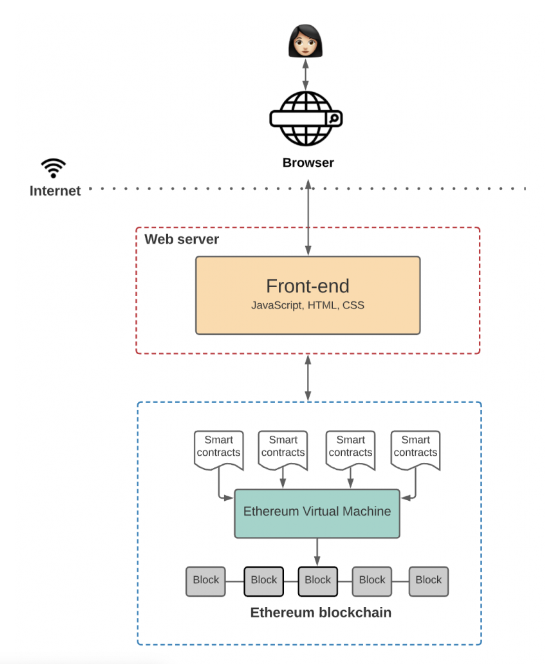
\includegraphics[width=12cm,keepaspectratio]{images/architecture_web3.png}
	\caption{Architecture Web 3.0 based on \cite{newstack}}
	\label{fig:architecture-web3}
\end{figure}

%\begin{figure}[H]
%	\centering
%		\includegraphics[width=12cm,keepaspectratio]{images/web3_architecture}
%	\caption{Web 3.0 Simple Architecture [source: author]}
%	\label{fig:web3-architekture}
%\end{figure}


From these definitions, it should be easy to see, that the Web 3.0 is still a work in progress.\\
To better understand what the Web 3.0 is, it is necessary, to look at the technologies which enable it. The focus of this Bachelor thesis lies on blockchain technologies, which will be presented and further discussed in the coming sections.


\newpage
\section{Technologies}
There are several aspects of blockchain technologies, which are used in the new generation of the web. In this section the core concepts of blockchain technologies will be presented.\\

\subsection{Blockchain technology}
The blockchain enables the decentralized part of the new generation of the web. The blockchain technology has gotten much attention in recent years, since the rise of cryptocurrency. The most popular implementation of a Blockchain is Bitcoin, which, at the time of writing this Bachelor thesis has a market capitalization of over 420 Billion Dollars, as stated on \href{https://www.coinbase.com/explore}{coinbase.com}.\cite{coinbase} Another popular blockchain technology is ethereum, with a market capitalisation of over 180 Billion Dollars.\cite{coinbase} In this Bachelor thesis, ethereum will be the distributed-ledger technology of choice, since it has very good documentation, is constantly improved and has a large community behind it.\\

Blockchain falls into a category of a distributed ledger technology. This technology can fulfill some of the goals of Web 3.0, because of its properties of a decentralised network, anonymity, persistency and auditability. A blockchain consists, as the name already suggests, of a sequence of blocks, where each block can hold a certain set of data. In the field of cryptocurrency, this data encompasses all the transactions that have been made with the currency.  \cite{blockchaingeneral}

\begin{figure}[H]
	\centering
		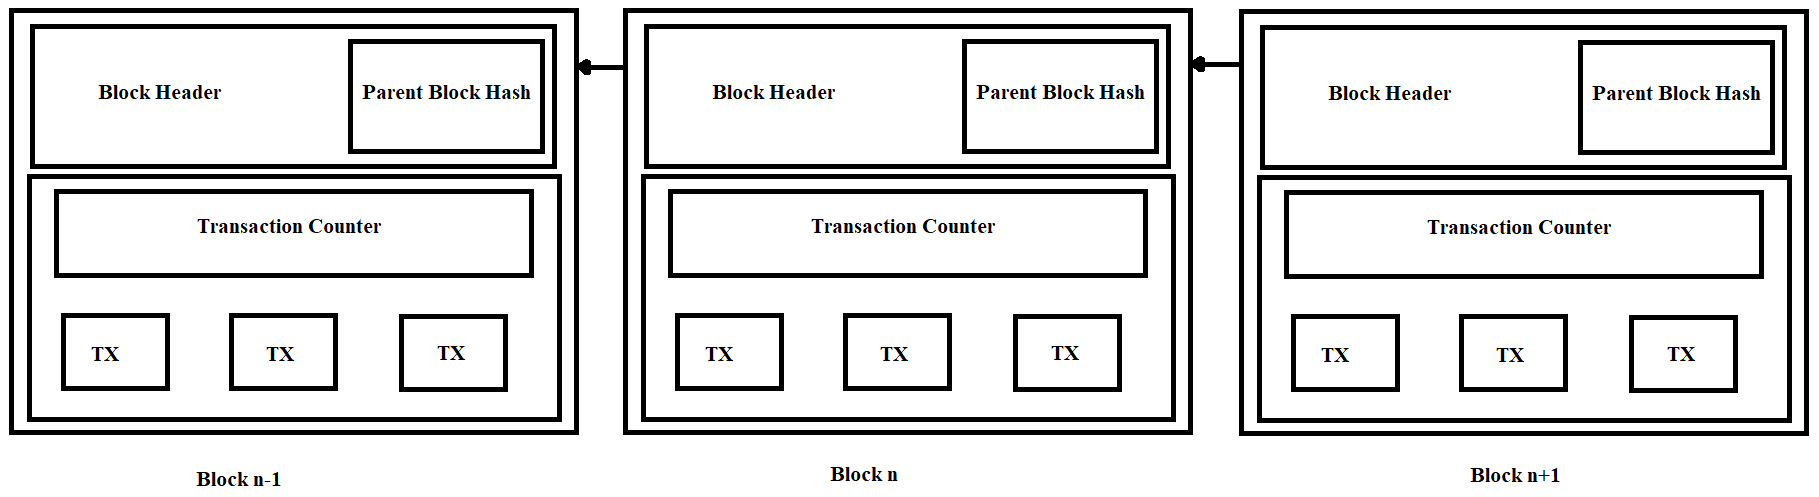
\includegraphics[width=15cm,keepaspectratio]{images/blockchain architecture.png}
	\caption{Blockchain Architecture from \cite{blockchaingeneral}}
	\label{fig:blockchain-architecture}
\end{figure}

The blocks of a blockchain differ with the specific implementation of a blockchain, however some basic elements are always roughly the same. In a blockchain each block has a reference to its parent/previous block, where the reference is in form of a cryptographic hash of a previous block, which is stored in the block header. A cryptographic hash is a sort of algorithm, that transforms a set of data into a string, that is always the same length. The reference to the previous block is always there, except for the first block in a blockchain (also called the genesis-block). \\
In Figure 2.3 an example of a blockchain architecture is depicted. The block header usually contains a version number, a timestamp, a field for the hashed value of all transactions contained in the block, a nonce - which is important for a security aspect of the blockchain, as well as creating new blocks, a field for the threshold of a valid block hash and as already explained, the parent block hash, which links the preceding block.\\
The decentralized part of the blockchain is then made possible by people who provide their own network bandwidth and computational power to the network. These people are called miners and represent the nodes of a network. The miners are responsible for adding new blocks to the blockchain. In the case of cryptocurrency, they are therefore responsible for the validation of transactions in the network. As a reward for the participation of miners, they get a certain amount of the cryptocurrency e.g. Ethereum, whenever a new block is created. The process of validating the blockchain is called the consensus process, in a public blockchain, each user can participate in this process.\\
The first, well known consensus strategy, which is also used in the Bitcoin network is the Proof of Work (PoW) strategy. This requires complex mathematical calculations to be done, which also creates a number of problems e.g. energy cost, that will be addressed in chapter 3.\\
Another strategy is the Proof of Stake (PoS) strategy, which addresses some of the problems of PoW, but introduces new problems of their own.\cite{blockchaingeneral}\\

There are four main categories, that a blockchain can fall into:\cite{geekstypesofblockchain}
\begin{itemize}
    \item Public blockchains - These blockchains are completely open and not owned by anyone. Every miner/node in the network holds a copy of the entire blockchain.
    \item Private blockchains - These blockchains are not open to anyone. The owners of such a blockchain can chose which people have permission to participate in the blockchain network.
    \item Hybrid blockchains - This is a mixture of a private and public blockchain.
    \item Consortium blockchains - This is a blockchain, that has multiple owners.
\end{itemize}

\subsubsection{Proof of Work}
PoW is a conses mechanism/system, which is used in many blockchains. It was first introduced in the Bitcoin blockchain. The peers/miners in a network can, so to speak, vote with their respective computing power, by solving mathematical problems and then creating the appropriate blocks of the blockchain. The miners have to find the correct nonce of value of a block. When this value is then hashed with additional block parameters the value of the resulting hash has to be smaller then the momentary target value. Once the correct nonce is found, the block is created and forwarded on the network layer to all the peers in the network. This block is then validated by the other peers in the network.\cite{pow2016}

\subsubsection{Proof of Stake}
The PoW mechanism has a high demand for energy among other shortcomings, which is why the PoS mechanism was developed.\\  
PoS is meant to reduce the computational power needed to solve mathematical problems. Instead of every peer in a network competing to solve the next block in a blockchain, to get the mining reward, a leader is selected based on their stakes. In cryptocurrency blockchain networks the stakes would be the number of coins in possession. This promises lower energy consumption, as well as a faster speed at which transactions are confirmed.\cite{pos}\\\\


Two further technologies, which are important and often found in combination with the term Web 3.0/blockchain technologies are smart contracts and DApps (Decentralized Apps). These will be presented in the next chapters.

\newpage

\subsection{Smart contracts}
The term "smart contract" was first coined in 1994 by Nick Szabo.\cite{ethereumsmartcontractsgeneral} He already foresaw a marketplace in the digital world, built on these processes/contracts.\\
The main idea behind smart contracts is to create a digital contract, without the need of a middle-man e.g. a lawyer, who ensures that the contract is not changed after all involved parties have agreed to the terms of said contract.\\
The clauses written in  a smart contract will be automatically executed, when certain conditions are met. This applies also if one of the parties involved in a smart contract breaches a clause, then said party will be automatically punished. In the case of cryptocurrency this means, that the party breaching the contract will be deducted a certain amount of coins, which is specified in the smart contract.\cite{ethereumsmartcontractsgeneral}\cite{smartcontracts2019}\\
This contracts are pieces of code, which run directly on a blockchain. In the case of the ethereum blockchain, as described on \href{https://ethereum.org/en/developers/docs/smart-contracts/}{ethereum.org} they are a type of an ethereum account themselves.\cite{ethereumsmartcontracts} This means, that the contract itself can be the target of a transaction and has an account balance. They are not controlled by a user, they rather run automatic, and execute the code according to their programming. An example for a smart contracts would be a vending machine, which operates as follows:\cite{ethereumsmartcontractsgeneral}
\begin{itemize}
    \item A product is selected
    \item The vending machine displays the cost of the selected product
    \item The amount to buy the product is inserted into the vending machine
    \item The program on the vending machine verifies that the inserted amount matches the cost of the product
    \item The selected product is dispensed
\end{itemize}
This example should show, that the product is only dispensed after all requirements have been met. Just like a vending machine a smart contract automatically checks, if all requirements have been met and then executes a specified part of the code.

\subsection{DApps}
Decentralised applications are built on decentralised networks. They work, by combining a smart contract and a user interface. This means that the business logic/the backend code of a DApp runs on the decentralised network and the frontend runs on the client. They have a certain set of characteristics, which can be described as follows:\cite{ethereumddapps}
\begin{itemize}
    \item The are decentralized, which mean that they run on a peer-to-peer network
    \item They are deterministic, that means that they always perform the same functions, regardless of the environment they are run in
    \item They are Turing complete, which means, that if enough resources are provided, they can perform any action
    \item They are isolated, that means that an error won't disturb the normal functioning of the network they are run in
\end{itemize}
\newpage
\chapter{Challenges of the Web 3.0}

There still are a multitude of challenges to overcome, before the Web 3.0 can be realised. The first challenge would be a clear definition of the term, which is not the case at the time of writing this Bachelor thesis, as already mentioned in section 2.2.\\
This section has a focus on the challenges blockchain technology has yet to overcome, before it can fulfill all the goals, which Web 3.0 promises. The paper "A Survey of Blockchain From the Perspectives of Applications, Challenges, and Opportunities" \cite{challengesandapplications2019} provides a great outline for the challenges blockchain technologies face. This Bachelor thesis will expand the outline with recent discoveries and other perspectives, as well as possible solutions to the challenges of the Web 3.0. In the following chapters, this Bachelor thesis will present challenges of blockchain technologies, such as energy consumption, performance and scalability, privacy and ownership, interoperability and Fairness and Security.

\section{Energy Consumption}
A major point of blockchain and Web 3.0 technologies is their energy consumption. Especially since the current energy crisis has already had an impact on miners of cryptocurrency\cite{guardianmining}. For many mining is not feasible anymore, since the energy costs already outweigh the returns miners get from creating new blocks. This in turn lessens the decentralization of a blockchain, since mining at this point is usually only possible for owners of large mining-farms.\\\\
The current used consensus algorithm in bitcoin is the PoW algorithm. This algorithm has already been proven to be highly unsustainable, as it consumes large amounts of energy to run. With a PoW algorithm many miners compete for creating a new block and appending it to the chain. A lot of computing power is lost through this competition. This lost computing power can be translated to lost electricity. Since global warming is on the rise and the need for renewable energy rises, this model for a consensus algorithm will not be fruitful in the long run. The website \href{https://ccaf.io/cbeci/index}{ccaf.io}\cite{cambridge} from the University of Cambridge offers a tracker for the energy consumption of bitcoin. The annualised consumption, at the time of writing this Bachelor thesis counts over 109 terawatt hours of electricity\cite{cambridge}. As a comparison, the country Austria with a population of nearly 9 million people as stated on \href{https://www.statistik.at/statistiken/bevoelkerung-und-soziales/bevoelkerung/bevoelkerungsstand/bevoelkerung-zu-jahres-/-quartalsanfang}{statistik.at}\cite{statistikaustriapop}, has a annual energy consumption of about 72 terawatt hours, as stated on \href{https://de.statista.com/statistik/daten/studie/325788/umfrage/stromverbrauch-in-oesterreich/#:~:text=Im%20Jahr%202021%20wurden%20innerhalb,der%20Kraftwerke%20und%20die%20Netzverluste.}{statista.com}\cite{statistakaustriaenergy}, at the time of writing this Bachelor thesis. The Cambridge Bitcoin Electricity Consumption Index \href{https://ccaf.io/cbeci/index}{ccaf.io}, also provides data about the greenhouse gas emissions, that are produced by the bitcoin network. The current estimate of annualised emissions are at over 55 megatons of carbon dioxide emissions. This further proves, that a new model for a consensus algorithm is needed, to be more efficient in terms of the energy needed to create new blocks and validate transactions.\\
An interesting comparison can be made, when bitcoin is compared against standard payment methods with fiat currency, such as a VISA credit card. The Bitcoin network uses far more energy per transaction then the VISA credit card. About 100 000 VISA transactions can be done for the energy cost of about one third of the amount that would be needed for a single Bitcoin transaction \cite{challengesandapplications2019}. 
The consensus algorithm that decreases the energy cost of transactions is the PoS algorithm. This is already implemented in the blockchain network known as ethereum. The ethereum network switched to the PoS mechanism on the 15th September 2022 \cite{ethereummerge}. They state that this switch reduced the energy consumption of the network by 99.95\% \cite{ethereummerge}. Ethereum merged its already existing blockchain with the "beacon chain", which already ran in parallel to the PoW ethereum blockchain, which ethereum had implemented thus far. They claim that no data has been lost after the merge and together with the reduced energy cost, they also claim to improve the scalability, security and sustainability of the network \cite{ethereummerge}. This could be a sustainable way to use blockchain technology in the future.

%https://ieeexplore.ieee.org/stamp/stamp.jsp?arnumber=8805074

\section{Performance and Scalability}
Since blockchain technologies have gained a huge amount of popularity in the recent years, a factor that needs to be considered is the performance of blockchain networks, as well as the scalability of the systems. The amount of data transferred daily over the world wide web is substantial and ever increasing as more and more users create and consume content. The questions is, if the blockchain technology can satisfy the expectations of users for a highly scaleable network with low latency and high throughput. The scalability trilemma states, that there is always a trade off between security, decentralization and scalability as is shown in Figure 3.1. This means, that not all of these three attributes cannot all be implemented at the same time, without one of these attributes being compromised. \cite{ethereumvision}

\begin{figure}[H]
	\centering
		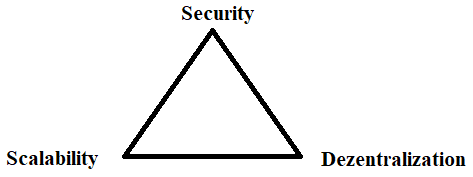
\includegraphics[width=10cm,keepaspectratio]{images/trilemma.png}
	\caption{Scalability trilemma based on \cite{ethereumvision}}
	\label{fig:scalability-trilemma}
\end{figure}

Another attribute that can be added to the trilemma, which would make it into a quadrilemma, is the aspect of trust, since blockchains, which have trusting parties may implement simpler consensus algorithms in order to achieve a better scalability. \cite{SANKA2021103232}\\

The PoW mechanism of Bitcoin for example offers a high scalability. The Problem is, that it suffers from low throughput as a result \cite{challengesandapplications2019}. This problem arises because a lot of computational power is wasted with the PoW algorithm when miners try to solve a cryptographic puzzle, to append another block to the blockchain and reap the mining rewards. The throughput of Bitcoin is only at about 6-10 transactions per second and a new block is added, on average, within a timeframe of 10 minutes \cite{challengesandapplications2019}. This creates huge problems, since it is far too slow to allow a large number of transactions to be processed in a reasonable timeframe. Another problem comes with the limited blocksize of a blockchain network. Bitcoin for example offers a blocksize of 1MB per block. This is done to make the blockchain more secure, but it reduces the amount of transactions, which can be written onto a block, making the network slower in the process.\cite{challengesandapplications2019}

Since the Ethereum network has switched from the PoW mechanism to the PoS mechanism, it offers many advantages over the traditional implementation, but there are also the known trade offs with the switch to the new consensus mechanism. As already mentioned, the cost for the energy consumption is highly reduced with the PoS algorithm. Another benefit is the higher speed of transactions. The Ethereum network, for example, promises thousands of transactions per second. Some argue, that the trade off with PoS algorithms is in the lessening of the decentralization of the network. However, ethereum claims, that that is not the case, since economies of scale do not apply to the PoS mechanism, as they do for the PoW mechanism, making the network more decentralized in the process.\cite{pos}


\section{Privacy and Ownership}
Another major point of the Web 3.0 and blockchain technologies is privacy. It is common knowledge, that big industries, such as Google collect user data in order to run their business \cite{nbcgoogle}. As the common saying goes "If there is no product, you are the product". One of the goals of the next generation of the web is to enable better privacy for the users of the web. A way to achieve this goal is with blockchain technologies. The idea behind using a blockchain to enable better privacy for clients, is to store data on the blockchain, rather than on a centralised database. This would mean, that data is then not owned by the owner of the database, but, in the case of a dezentralised network, the data is owned by the creator of the data. However, as already mentioned in the previous chapter, storing the entire content of a website in the blockchain is not feasible because the blocksize in a blockchain is limited and cannot allow for all data to be hosted on-chain.\\\\

The paper "Decentralizing Privacy: Using Blockchain to Protect Personal Data" \cite{privacy} proposes a solution to this problem, which will be further explained in this chapter. The main aspects of the proposed solution are as follows:
\begin{itemize}
    \item Data Ownership - Each user in the system owns and controls their personal data.
    \item Data Transperency and Auditability - There is complete transperency over which data is collected from each individual user and how this data is accessed
    \item Fine-grained Access Control - For mobile users it is often the case, that once the access to personal data is granted, the permission to use said personal data cannot be reverted. Access control addresses this issue, by giving users the possibility to revoke these permissions.
\end{itemize}
The entities in the proposed solutions are mobile phone users, that want to download data and use applications / services. The miners/nodes are entrusted with the maintenance of the blockchain and with storing the key-value data. In return for their provided computational power, they get certain incentives. The system works by implementing two new types of transactions, namely \( T_{access} \), which is, as the name suggests used for access management and \( T_{data} \), which is used to store data and retrieve it. To better understand this solution an example is provided. A new user, who wants to preserve their privacy, downloads an application that uses the platform proposed in the solution. At the first sign up, the platform generates a new identity and sends it, together with all relevant permissions, to the underlying blockchain, in a access transaction. The data that is sent is then encrypted with a shared key and sent to the blockchain via a data transaction. Then the identity is routed to an off-blockchain key-value store. Only a pointer to the data is stored on the blockchain, which is a hash of the data. This is important, because it means, that only a small amount of data needs to be stored on-chain, while the majority of the data is stored off-chain, which tackles the problem of on-chain data storage described earlier in this chapter. After the user is thus integrated in the system, both the user and the service can now query the data by using the earlier mentioned pointer to the data. For the service, the permissions to access the data are checked as well, to ensure that only authorized access is granted. The user can later change the permissions to access their data at any time by using a access transaction.\cite{privacy}

This could be one possible solution to enable better privacy for the users of the world wide web and ensure, that private user data is not accessed without permission.

\section{Interoperability}
Another big topic when it comes to blockchain technology is the interoperability between different implementations. At the time of writing this Bachelor thesis there are already a multitude of different blockchain implementations. The exact number of how many blockchains there are is uncertain, but it can be estimated that there are more than thousand, maybe several thousand implementations of blockchains out there. Thus far, there is no standardised protocol, that enables different blockchains to communicate and operate with each other. The main application of blockchains today is the mining and trading of cryptocurrencies. Arguably, there is some interoperability provided for cryptocurrencies, since they can be exchanged for one another on sites such as \href{https://www.coinbase.com/}{coinbase.com}. However, as far as other Web 3.0 applications are concerned, there is still no standard, through which interoperability can be achieved. \cite{challengesandapplications2019}\\

The paper "Make Web3.0 Connected"\cite{connected2022}, has its focus on the problem of interoperability and will be further discussed in this section.

The paper defines three infrastructural enablers for the Web 3.0:
\begin{enumerate}
    \item Blockchains, through this technology verifiable computing can be supported
    \item Federated / centralised platforms, these should be able to publish verifiable states, because some functionalities are difficult to implement on a blockchain
    \item A secure platform, which serves as a connection between blockchains and platforms
\end{enumerate}

The focus of the aforementioned paper lies on the third enabler of the Web 3.0, the platform that should connect different blockchains and platforms. They call their interoperability platform the "HyperService". This platform would be powered by a new programming framework: The HSL (HyperService Programming Language) programming language, for writing cross-chain DApps and by UIP (Universal Blockchain Interoperability Protocol), which realizes the operations that are defined in DApps.\cite{connected2022}\\

This new technology could make the interoperability between different blockchains possible. If it gains popularity and becomes a standard in the field remains to be seen.

\section{Fairness and Security}
As well as every other technology, that is used on the web, blockchains are also prone to cybersecurity attacks. To mitigate such attacks is always difficult, since it is impossible to foresee all possible angles of attack. Especially in cryptocurrency implementations of blockchains, such attacks could be devastating, since users would not only lose data, but valuable assets as well.\\
A well known and widespread attack on blockchains is the so-called 51\% attack. This attack works, if a attacker or a group of multiple attackers gain a majority of the blockchains hashrate. Once the majority is achieved, the attackers can change vital data that is stored on the blockchain. Another angle of attack is called "Selfish mining", this is done by mining pools, which consist of several miners, that are joined together to mine blocks more efficiently. The attack works by waiting before broadcasting a successfully mined block to the entire network. The attackers can mine additional blocks, while regular miners still try to mine a previous block on another branch of the system. Once certain criteria are met, the attackers broadcast the mined blocks to the rest of the network. Their blocks get accepted, because they have a higher complexity and length than the blocks of regular miners. This can lead individual miners to join the malicious mining pool in order to not be excluded from reaping the rewards of mining. While these attacks still exists, popular blockchain networks such as ethereum have already implemented some countermeasures for selfish mining, especially through the change to PoS.\cite{challengesandapplications2019}\\

Another attack angle are the smart contracts, which are implemented on the blockchains. The contracts may be advertised as more secure than having a middleman, yet they are not immune to bugs and implementations that can be exploited. The biggest such hack was, when the DAO (Decentralised Autonomous Organization) \href{https://www.geeksforgeeks.org/daodecentralized-autonomous-organization-in-blockchain/}{geeksforgeeks.org}, that used the ethereum network was hacked because of a bug in a smart contract. This severely impacted the price of the ethereum currency and also raised questions on the security of blockchain networks.\cite{geeksDAO}\\

These are just some of the security issues that blockchain technology faces. As already stated, it is not possible to foresee every possible attack that can be done, it is rather an incremental process to harden the security of a system.


\newpage
\chapter{Opportunities of the Web 3.0}
This chapter will present the opportunities of the Web 3.0 and therefore the many different fields of applications for blockchain technologies. As already mentioned, cryptocurrencies, such as ethereum and bitcoin are one field of application for blockchain technology, however they are not to be confused with the term blockchain itself.

\section{Energy sector}
The application of Web 3.0 and blockchain technologies in the energy sector is not meant to improve the harnessing of electrical power itself. As already mentioned in chapter 4.1, blockchains consume a lot of energy and are therefore not a model that reduces the amount of energy needed for a system to run. However, PoS blockchains already take a step into the direction of reducing the amount of energy needed to run a blockchain and that at a significant level. The application of blockchain technologies in the energy sector is rather focused on the management of a distributed market. With more and more people investing in, for example, the photovoltaic industry, the management of these widespread entities has become a non-trivial task. Here blockchain technologies could provide a better way to store and manage data in the energy field, than a regular centralised system. Blockchain technology would especially be useful to ensure the transparency and the management of data access of a energy system, as well as proper voltage control of the system. There is a proposal for a system, that has these properties, which makes use of a mixture of a public and private blockchain. The public blockchain would be needed to ensure transparency in the system, to store data and to verify the consistency of the system. It would be responsible for ensuring security and the integrity of data. The private blockchain on the other hand, would be needed to verify the accuracy of transactions. As already mentioned, another application could be the control of the decentralised energy-grid.This relates to the problem of how users of photovoltaic energy need to upload their generated excess power to their local energy grid. This process needs to be managed carefully in order to prevent energy spikes on the grid, which can lead to a variety of problems. Therefore the power that is produced by decentralised entities needs to be regulated in a meaningful way. This can be achieved through the use of smart contracts on a blockchain. The contracts themselves could be programmed in a way that selects nodes of the blockchain network to act as a regulator for the voltage during a certain control period. The benefit, in comparison to a centralised system, would be that there is no need for a separate entity that is responsible to control the voltage, since the smart contract would take care of the problem. This approach is based on a private blockchain and therefore not free of the limitations of such a system. Another proposal for energy management, would be the implementation of a smart grid. This would offer a lot of benefits for consumers, since they could manage their own individual energy supply and sell their surplus energy as they see fit. In this system, they would gain a certain amount of a cryptocurrency, for the sale of their energy. The main functions of this project would be the recording of data that is generated when energy is traded and to control the energy that is generated.\cite{energy}

\section{Healthcare}
The healthcare sector needs to manage large amounts of data to keep track of patient related personal information, as well as medical records. The problem with the current centralised systems, which manage such data, is that they could pose the danger of being a single point of failure. Another problem is that many different medical institutions manage their own data, which creates lots of duplicated information and discourages collaboration. A further problem, is the need for privacy and data ownership of medical records. Blockchains, with their inherent properties of being a network that promotes security, privacy and transparency could lead to a better governance of data in the healthcare sector. This section will present some of the possible applications and solutions to the aforementioned problems.\\
One of the most popular applications of blockchain technologies in the healthcare sector is the management of patient data. As of now, this information is usually managed by humans, which can lead to mistakes and inconsistencies, that are produced by human-error. Often a separate entity, such as a insurance department is needed as well. This leads to an increase in the time it takes to access needed medical records, as well as an increase in the complexity of the system. To administer the proper care and treatments for individual patients with different medical histories is crucial. The information needed to administer the correct treatment of a patient could be stored on a blockchain to reduce the amount of duplicate information. Duplicate information is for example generated whenever a patient switches to a different medical institution, where they have to enter all their personal data again, which produces additional costs. A blockchain network which has proper access protocols configured, could make it possible for many health professionals to access the information of a patient without the need to generate this data anew. Costs in the sector would therefore be reduced, since tests from many different facilities would not have to be repeated. Smart contracts can be used to ensure that only authorized access is granted and that data is not used or accessed in a malicious way.
Another application in the healthcare sector is the management of the drug supply chain. There are lots of low quality and counterfeit drugs circulating around the world. Blockchain technologies could be used to monitor the distribution and production of drugs on a supply chain. This would help to make the whole process more transparent and to detect modified or altered drugs. The immutability and timestamps of a blockchain would ensure that the data, that is saved on the blockchain, cannot be modified and would therefore increase the security of the system.
Another benefit of the blockchain in the medical sector would be to further improve the collaboration of researchers in the field. The blockchain could make the data collection, which is collected in the process of clinical trials, more trustworthy. The technology would also ensure the integrity of the provided data and help to reduce the amount of incorrect data.
Through smart contracts and the use of cryptographic keys (e.g a private and a public key), the access to medical records of a patient can be better managed. For example in the case of a medical emergency it is crucial, that the medical data is readily available to the healthcare professionals which administer the treatment. In such a scenario time is of the essence and proper access and permission management can lead to a significant reduction of the time that is needed to access such records, as well as save the life of the patient.\cite{medicalsector}\\

These are just some of the benefits and possible applications of using blockchain technology in the healthcare sector.

\section{Voting}
In many countries the voting process is still far from being fully digitalized and relies on the honesty and collaboration of human examiners. This produces significant costs, since a lot of the analysis of individual votes must be done by hand and it is prone to human-error. Voting fraud is still a major issue, especially when voting relies on the use of centralised systems that are operated by members of a specific government party. This allows for backdoors in voting systems, that can be exploited and can change the outcome of an election and therefore the future of a country. Blockchain technology can offer benefits to a voting process, because of the immutable nature of the technology.\\
One approach that can be used to get to a decentralized voting system is described in the paper "De-Centralized Voting System using Blockchain"\cite{voting}. In this paper a centralised server is used to manage the verification of eligible voters. To enhance the security of the system, two-factor-authentication is used in the approach. Then they propose a framework, that is divided into three phases. The phases are the Pre-Election, the Election itself and the Post-Election.
\begin{itemize}
    \item Pre-Election Phase - Here a smart contract is created with all the necessary details of the current election. Then election organizers can register new voters or invite existing voters to cast their vote. It is necessary, that every voter has an unique id, which is assigned by the platform. After a voter is verified as eligible to vote in an election, their respective wallet address is added to their voter data.
    \item Election Phase - In this phase voters can cast their vote via a transaction to the blockchain network. It is notable, that a vote count and data for analysis on the current election can be retrieved at any time using special view methods in the smart contract.
    \item Post-Election Phase - This is the last phase of the process, here the window, which allows for voting is closed and all ids of registered voters are made public, along with the results of the election.
\end{itemize}
The proposed approach uses 4 modules. These are the smart contracts, that are created for each individual election, a central server that is used to manage the authentication of the voters, a user interface for voters and a Organisation Server that is managed by the organizers of an election. A architecture, that depicts how such a voting system could look like, is depicted in figure 4.1. \cite{voting}

\begin{figure}[H]
	\centering
		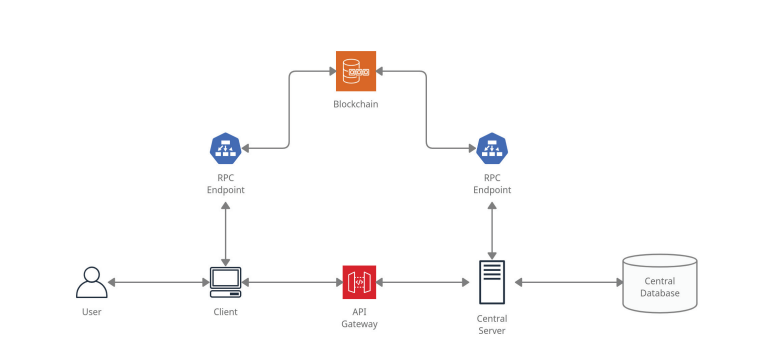
\includegraphics[width=17cm,keepaspectratio]{images/architecture_voting.png}
	\caption{Architecture for a voting system from \cite{voting}}
	\label{fig:architecture-voting}
\end{figure}

\section{Identity Management}
Another useful application of blockchain technologies is to use them as a tool for verifying the identity of a person. Ownership of personal information is a big topic, especially with how private data is treated currently. If a user registers to a site with a centralised server, the personal information of the user is often handled in a way, that is neither conform with current regulations, nor does a user have full control over how their data is passed to other sites or entities. Blockchain technologies can address these problems. The benefit of a blockchain being immutable and transparent can make it possible for every user to see exactly, which data of the user has been accessed. Other benefits would be, that permissions regarding who can access private information can be changed and that data is owned by the user, rather than by an organisation.\\
The paper "BIdM: A Blockchain-Enabled Cross-Domain Identity Management System" \cite{identity} describes a system, which can improve the management and privacy of personal data. The proposed solution in the paper has the following functions:
\begin{itemize}
    \item Identity registration - At registration a public key is provided then the specified identifier is bound to it
    \item Identity Update - The relationship between the public key and identifier is updated
    \item Identity Authentication - Check if identifier and public key match
    \item Identity Revocation - the identifier is unbound from the public key
\end{itemize}
With these functions and their proposed solution a cross-domain identity management system can be realised.\\
If this implementation gains popularity and is further developed to be used as a Web 3.0 technology remains yet to be seen.\\\\

This concludes a short overview of some of the blockchain technology applications, that could be implemented in the Web 3.0. This is, of course, just a small subset of all Web 3.0 applications that are currently discussed and further research is needed in many fields until these applications are fully functional and can be used for daily tasks in the next generation of the web.

\newpage
\chapter{Conclusion}
The web is continually growing and new technologies emerge often. There have been many changes since the web 1.0 was first released. The current web 2.0 focuses on "rich user experiences" and social media. Here the user is the center of the web, with the ability to create and consume content. The Web 3.0 is still in need of further improvements. As of now, there is no clear definition for the term itself, though it is clear that decentralization, immutability and privacy play a huge part in it. With blockchain applications these goals can be achieved, however this technology has still got to face many challenges. The problem of the high energy consumption, which stems from the PoW mechanism, has been vastly improved on by switching to the PoS mechanism. There are other aspects, such as the problem of scalability and the interoperability between different implementations, that have seen improvements over the last years, but still need work, before they can be properly implemented. The applications of the technology seem vast. Some of them are the improvement of management systems, for example in the energy and healthcare sector. Others can be found in the privacy and security sector. An example would be to improve the government of user data and minimise voting fraud. It can be said, that there are still a multitude of challenges to overcome, before the Web 3.0 can be realised.

\newpage
\chapter{Future work}
This Bachelor thesis can lead to a better understanding of the Web 3.0, blockchain technologies and the challenges and opportunities thereof. A better definition of the next generation of the web can be developed to make it easier to understand. The presented challenges in this Bachelor thesis can lead to further improvements of the blockchain for general purposes. The energy cost of blockchain networks could be reduced and the security could be fortified against malicious attackers. This Bachelor thesis can spark new ideas for the applications of blockchain technologies in many different areas.


\newpage
\chapter{Summary}
This Bachelor thesis offered a brief introduction into the Web 3.0 and its respective challenges and opportunities from the perspective of blockchain technologies. It offered a brief history of the web from web 1.0 to the Web 3.0. The first web consisted mainly of static pages and was regarded as a read-only web, whereas the second web was considered as a dynamic web with read and write access. Then many different definitions of the Web 3.0 were presented, as of now, there is no clear definition, that has emerged. The blockchain technology and other constructs that are built on this technology, were presented, such as smart contracts and DApps. After that the Bachelor thesis presented different challenges and opportunities of the blockchain. Some major challenges are the energy consumption of blockchains, the trade-off between security, decentralization and scalability, privacy, interoperability between different implementations of blockchains and fairness and security. The possible applications of blockchains are manifold and just some of them were presented in this work. The applications can be found in fields, such as the energy and the healthcare sector, voting and identity management. 

\newpage

% --- Bibliography ------------------------------------------------------

%IEEE Citation [1]
%\bibliographystyle{IEEEtran}
%for alphanumeric citation eg.: [ABC19]
%\bibliographystyle{alpha}

% List references I definitely want in the bibliography,
% regardless of whether or not I cite them in the thesis.

\newpage
\addcontentsline{toc}{chapter}{Bibliography}
\printbibliography
\newpage

% --- List of Figures ----------------------------------------------------

\addcontentsline{toc}{chapter}{List of Figures}
\listoffigures


% --- List of Tables -----------------------------------------------------

\newpage
\addcontentsline{toc}{chapter}{List of Tables}
\listoftables

% --- Appendix A -----------------------------------------------------

\backmatter
\appendix
\begin{appendices}
\chapter{Appendix}

(Hier können Schaltpläne, Programme usw. eingefügt werden.)

\clearpage
\end{appendices}

\end{document}
